\documentclass[a4paper, 11pt]{report}
\usepackage[english]{babel}
\usepackage{microtype}
\usepackage{amsmath,amssymb}
\usepackage{amsthm}
\usepackage[round, authoryear]{natbib}
\usepackage[all]{xy}
\usepackage{graphicx}
\usepackage{framed}
\usepackage{enumerate}
\usepackage{qtree}
\usepackage{mdframed}
\usepackage{algorithmic}
\usepackage{algorithm}
\usepackage{tikz-dependency}
\usepackage{float}
\usepackage[OT2,T1]{fontenc}
\newcommand\textcyr[1]{{\fontencoding{OT2}\fontfamily{wncyr}\selectfont #1}}
\bibliographystyle{plainnat}
\author{}
\title{}

%Define theorem style for definition and metric
\theoremstyle{definition}
\newtheorem{metric}{Metric}
\newtheorem{notion}{Notion}
\theoremstyle{plain}
\newtheorem{definition}{Definition}
\def\citepos#1{\citeauthor{#1}'s (\citeyear{#1})}

%Define new float environment for tables that is boxed
\floatstyle{boxed}
\newfloat{tab}{tbp}{lop}
\floatname{tab}{Table}


\begin{document}
\maketitle
\tableofcontents



%%%%%%%%%%%%%%%%%%%%%%%%%%%%%%%%%%%%%%%%%%%%%%%%%%%%%%%%%%%%%%%%%%%%%%%%%%%%%%%
%%%%%%%%%%%%%%%%%%%%%%%%%%%%%%%%%%%%%%%%%%%%%%%%%%%%%%%%%%%%%%%%%%%%%%%%%%%%%%%

\chapter{Introduction}

%%%%%%%%%%%%%%%%%%%%%%%%%%%%%%%%%%%%%%%%%%%%%%%%%%%%%%%%%%%%%%%%%%%%%%%%%%%%%%%
%%%%%%%%%%%%%%%%%%%%%%%%%%%%%%%%%%%%%%%%%%%%%%%%%%%%%%%%%%%%%%%%%%%%%%%%%%%%%%%

% Introduction to machine translation, quote Warren Weaver

\begin{quote}
\textit{When I look at an article in Russian, I say: `This is really written in English, but it has been coded in some strange symbols. I will now proceed to decode.}
\end{quote}

Evidently, automatic translation is not as easily solved as Weaver thought at the time. Over 60 years later, the state-of-the-art systems are still not able to produce translations of an arbitrary text with a quality comparable to that of a translation of a human translator. This was not for the lack of trying, on google.scholar one can find maar liefst .... articles with ``Machine Translation" in the title (and ... with ``machine translation'' in the document), in which many different methods have been explored. This work focuses on one such method: compositional translation. The compositional approach to translation is intuitively attractive, as it touches the fundamentals of semantics. As we are able to infer the meaning from a sentence by considering the words in it and the structure blablabla.... it seems reasonable to regard translation as a ...

suming we can infer the meaning of a sentence using the words in it and 



%Describe compositional translation
%Explain why compositional translation is attractive from a theoretical point of view.

In many fields in which translations occur (computer science, logic, philosophy), computational translation is a very common method. The semantics of an expression in a certain logic, for instance, can be unambiguously determined by considering the terms and the methods used to combine them. Translating such an expression into another logical language can be effectively carried out by translating these terms and methods into the terms and methods particular for the second logic.

%Explain why for language it is not so straight forward that we can do this: words have multiple meanings, sentences are vague and ambiguous, building blocks unclear
%Explain that we also do not a-priori dispose over grammars and mappings, as we did not design natural languages as artificial languages, nor is it clear of such mappings even exist.


% although not every grammar is suitable for compositional meaning assignment, the class of languages that can be analyzed is not restricted, nor are the meanings that can be assigned: any recursively enumerable language can be generated by a compositional grammar, and any semantics can be dealt with in a compositional way. 
%Is this helpful? Is NL recursively enumerable? What about ambiguity

However, none of this teaches us if compositional translation is a reasonable strategy for translating natural language. Intuitively, it seems reasonable that 'who-did-what-to-whom-relations' are universal for languages, but exploiting this fact in translation has proven to be a non-trivial task. The present work does not aim to develop a model for compositional translation of language, but rather attempts to empirically analyse if it is realistic to aim for one.\\
%Explain how this question becomes practical
Although this question is of theoretical nature, blabla explain that we have to deal with data such that it merely transforms to the question: can we find compositionality in the corpora we are training on, that an be of use in translation models. We will therefore also pay some attention to the use of the results, and make suggestions for future work.


\section*{Thesis Outline}

%Rewrite this when the rest is written
As mentioned before, the primary goal of this thesis is to investigate whether predicate-argument relations are preserved during translation. To do so, a tree will be searched that respects both the alignment (completely) and as much of the predicate-argument relations present in the source sentence as possible. The resulting tree will be scored according to how many of the predicate argument relations were allowed by the alignment, thus yielding a compositionality measure for the sentence.\\
The following chapter will give some theoretical background: it will explain the notion of alignment-respecting trees (anders) and provide some information on the grammar formalism used to extract predicate-argument relations.\\
Chapter give more information on the implementation of the research, while the actual experiments and their results will be presented in chapter 
%We probably also need a section about compositionality (lets see how that is gonna fit in)
%Describe the rest





%%%%%%%%%%%%%%%%%%%%%%%%%%%%%%%%%%%%%%%%%%%%%%%%%%%%%%%%%%%%%%%%%%%%%%%%%%%%%%%%%%%%%%%%%%%%%%%%%%%%%%%%%%%%%%%%%%%%%%%%%%%%%%%%%%%%%%%%%%%%%%%%%%%%%%
%%%%%%%%%%%%%%%%%%%%%%%%%%%%%%%%%%%%%%%%%%%%%%%%%%%%%%%%%%%%%%%%%%%%%%%%%%%%%%%%%%%%%%%%%%%%%%%%%%%%%%%%%%%%%%%%%%%%%%%%%%%%%%%%%%%%%%%%%%%%%%%%%%%%%%
%BACKGROUND ON MT AND TRANSFER MODELS

\chapter{Background}

Machine translation (MT) is a very complex problem, for which many approaches have been tried. In this thesis we focus on one such approach: the transfer method. More precisely, we are interested in \textit{statistical} models using this method. As discussing one particular method without as much as mentioning other possibilities seems a bit silly, we will start with a brief introduction to transfer models and statistical models. The most important sections of this chapter are section \ref{sec:theory} and \ref{sec:main}, in which, respectively, the main assumptions underpinning transfer methods and a number of proposed statistical models using transfer are discussed. The first two sections are introductory sections on early transfer models (\ref{sec:intro}) and statistical machine translation (\ref{sec:SMT}), and might be superfluous by readers familiar with the field. The chapter will be concluded with a short summary.


\section{A brief Introduction to Transfer Models}
\label{sec:intro}

The research field of machine translation arose almost immediately after the emergence of the first computers, and was one of the very first problems to be tackled by them. In the earliest approaches, sentences were treated as structureless sequences of words that could be translated more or less directly to a sequence of words in another language. The early models using such a direct approach are now called the first generation models. Such models, which ignore all structural aspects of the sentence, as well as relations between words, are clearly only suitable for languages that are structured almost identically, as translations whose structure deviates in any aspect from the original source structure will never be found. Most languages, if not all, are not this similar, and the direct approach of the first generation models was not very successful, leading to translations that are incomprehensible, not fluent en often not even meaning preserving.\\
The models that arose after the first generation, appositely called second generation models, aimed at translating structural representations of sentences, rather than translating sentences directly. In such a model, a source sentence is analysed into an intermediate representation that somehow conveys the semantic structure (or `meaning') of the sentence. This representation is mapped to a target side structure, that is then used to generate a target sentence. The process of mapping representations in one language to representations in another language is called transfer. A graphical representation of this process is shown in Figure \ref{fig:triangle}. 

\begin{figure}[!ht]
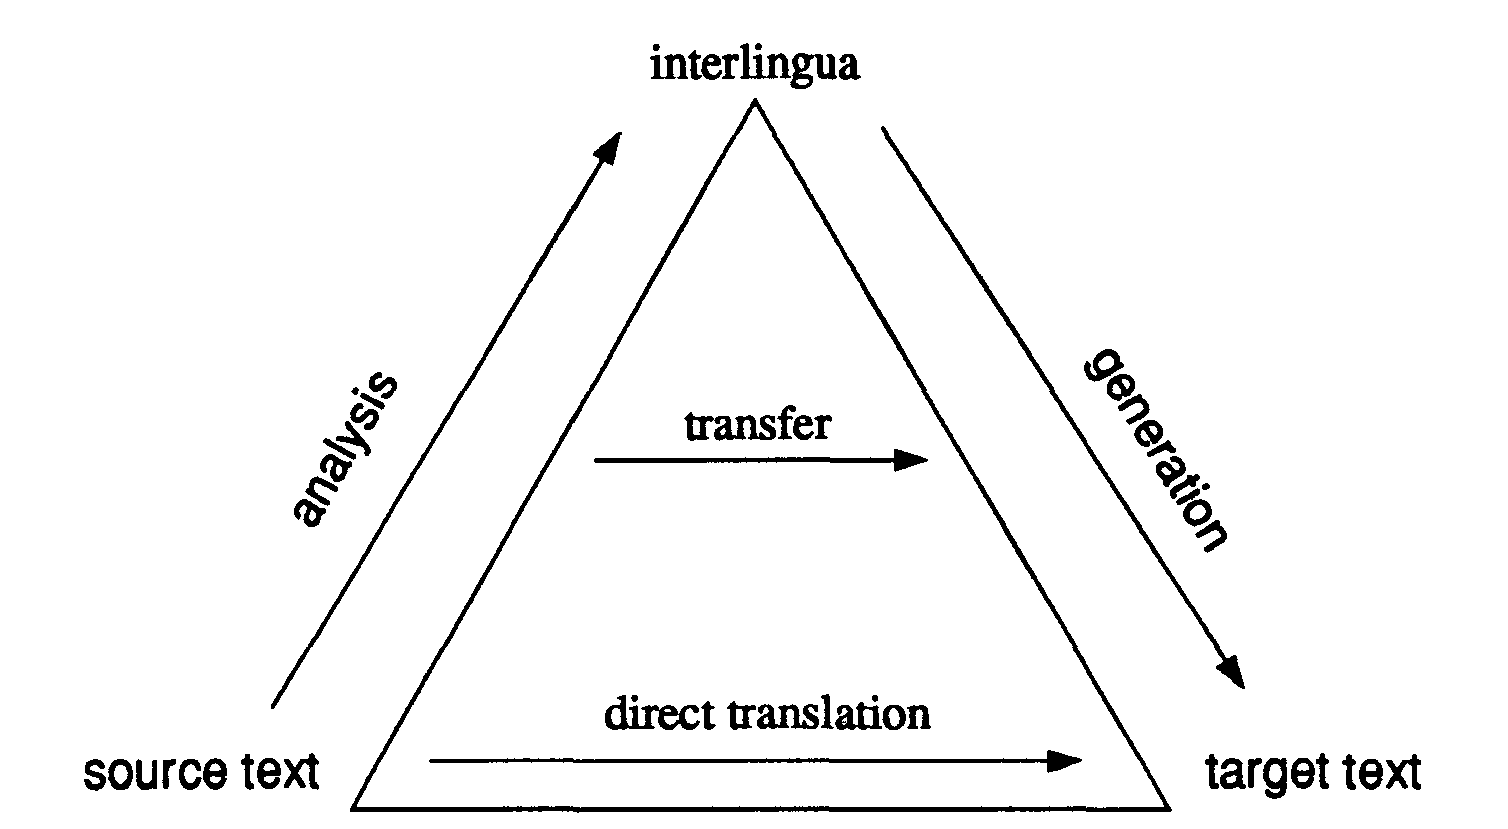
\includegraphics[scale=0.2]{translation_triangle.png}
\caption{Vauquois pyramid?}\label{fig:triangle}
\end{figure}

The depicted pyramid shows that the transfer method can be employed in different ways, varying the distance from source and target text to intermediate representation (analysis and generation, respectively). Direct translation is from this perspective just a transfer process in which the intermediate representation is identical to the sentence, and analysis and generation are both zero. Another extreme of the transfer method is the case in which the representation is a universal one, independent of natural language (called `interlingua'). In this case, the structural representation might be quite far from the original sentence, which makes analysis and generation hard, but the mapping part is reduced to the identity mapping.

\section{Statistical Machine Translation}
\label{sec:SMT}

Like the MT-world did, we will make a detour to statistical models. Driven by the thought that translation is too rich to formalize, the MT-world left linguistically motivated models for what they were, concentrating on models
that were based on information found in parallel corpora. Later, the two lines of models came together, and models that used earlier techniques in a corpus-based framework started to be developed. In this section we will briefly introduce the main concepts and thoughts behind models that use corpora to learn the parameters of their models.

\subsection{Word-based models}
The first working statistical MT model, inspired by \citepos{weaver1955translation} idea to use information theory to achieve automatic translation, was presented by \cite{brown1990statistical}. The paper was based on earlier work of the same research group \citep{brown1988statistical} and was further developed in a later paper \citep{brown1993mathematics}. Their models, now known as `IBM model 1-5', were intrinsically word based, and followed the noisy channel approach, modelling the probability $P(t|s)$ that $t$ is the translation of $s$.\footnote{In the literature, this probability is often expressed as $P(e|f)$, as the first IBM models modelled translation from French to English. However, this can be quite confusing for the reader, and in this paper we will stick to the more general $t$ for target and $s$ for source.} This probability is then expressed using Bayes' theorem resulting in the following expression (called ``The Fundamental Equation of Machine Translation" by the authors) for the desired translation $\hat{t}$:

\[
\hat{t} = \operatorname*{arg\,max}_t P(t)P(s|t)
\]

This equation splits the translation task in two: modelling the translation probability $P(s|t)$, and modelling the language probability $P(t)$. The model for $P(t)$, that is often an n-gram model, accounts for fluency and grammaticality of the target output. The generative model is standard in information theory, the crux of the model resides in how $P(s|t)$ is modelled. In the IBM models, this distribution is modelled by marginalizing over all possible ways in which the words in $t$ could have been generated by the words in $s$, thus $P(s|t) = \sum_a P(s,a|t)$, in which $a$ describes the mapping from target to source words. The 5 IBM models differ in the complexity of the approximation of the conditional probability $P(s,a|t)$, ranging from a very simple distribution in which $a$ is not considered at all (in which case the probability is independent of word-order) to rather complex ones in which $a$ is dependent on several parameters (details can be found in \cite{brown1993mathematics}).\\
All IBM models require a lexical translation probability (i.e., a dictionary-like function that specifies the probability of word $w_s$ translating into $w_t$. These probabilities are not directly observable from the parallel corpus (as the corpus is sentence aligned but not word aligned) and are learned from the data applying the expectation maximization algorithm, that has been proved to converge to a global optimum. Nowadays the IBM models are outperformed by newer sophisticated models and not in use any more, but their techniques for generating word-alignments are still used often to analyse translation data or to generate training data for newer models.

\subsection{Phrase-based Models}

The statistical IBM models still had the same drawbacks as the first generation of direct translation models: no structure of local context was considered and a large amount of natural language phenomena could therefore not be accounted for. With the introduction of (non linguistic) phrases as basic units in translation models 
(\cite{wang1998grammar,och1999improved}??) a major leap forward was taken towards a proper treatment of these problems. A phrase translation pair is a pair of contiguous source and target sequences such that the words in the source phrase are aligned only with words in the target phrase, and vice versa. \citep{och2004alignment}. Phrases are thus not restricted to linguistic phrases, but can be any arbitrary contiguous sequence of words. Keeping the architecture (more or less) the same, using phrases instead of words as translation units allows the model to use local context during translation. Phrase-based translation models can therefore capture short contiguous idiomatic translations, as well as small insertions and deletions and local reordering. E.g. both `a casa' and `o casa' are reasonable word-for-word translations of the English phrase `the house'. However, `o casa' is not a grammatical string in Portugese. The latter observation could be easily captured by a phrase-based model, as `the house' could be translated as one unit, but would be much harder to model in a word-based model. Furthermore, a word-based model would never be able to get the correct idiomatic translation of a phrase like 'kick the bucket', while a phrase-based model would have little trouble finding this translation (provided this specific idiomatic phrase was present in the training corpus).


\section{Transfer Models in Theory}
\label{sec:theory}

After having introduced both transfer methods and statistical methods, we will continue by discussing the transfer method on a more theoretical level. Intuitively, it seems very reasonable that we should be able to translate from one language to another by considering structural meaning representations of sentences and mapping the representations of one language to the representations of another language, but many implicit assumptions are made in the process. It is not hard to identify the two main assumptions underpinning the transfer method. As it aims to find structural representations and a mapping between them, it must thus assume that 1. such structural representations (however abstract) exist, and 2. a mapping between them exists. In this section we will elaborate on these assumptions (in the order we presented them), and discuss their fitness for MT-models. We will use examples from artificial languages, in which compositional translation is a very common method, to illustrate our arguments.

\subsection{Compositionality of Natural Language}

Most artificial languages have a method for structurally deriving the meaning of their expressions. For instance, the meaning of an expression in a logical language can be unambiguously determined by considering the atoms and the rules used to combine them. Consider for instance the expression $p\lor q$ in propositional logic, whose truth-value can be determined by plugging the truth values of $p$ and $q$ into the rule of the $\lor$-connective. Also programming languages can be interpreted by considering their basic units and the rules used to combine them. This property is called `compositionality' and is described in the following principle, that exactly matches the first assumption made in transfer models:

\begin{quote}
\textbf{The Principle of Compositionality}\\
The meaning of an expression is a function of the meaning of its parts and the syntactic rule by which they are combined \citep{partee1984compositionality}
\end{quote}

In linguistics there is no consensus about the extent to which natural language can be said to be compositional. Although the compositionality of some parts of natural language is undeniable for everyone - we can understand sentences we have never heard before because we know the words in it and are familiar with the methods that can be used to combine them - many have argued against compositionality of natural language as a whole (refs?). A detailed discussion of compositionality will not contribute much to this thesis, which we will make plausible (?) by discussing two important counter arguments and arguing why they are not of much relevance to the MT world.\\
Firstly, let us consider idiomatic expressions. Idiomatic expressions are an often heard argument against compositionality, as their meaning can clearly not be derived from its words and internal structure. For instance, there is no compositional analysis of the phrase `John kicked the bucket.' that leads to the conclusion that John died, even though this is certainly a possible interpretation of this sentence. The reason that such convincingly non-compositional expressions are not without further ado convincing arguments against compositionality is that the compositionality principle is not very well specified. That is to say, the power of a compositional grammar depends greatly on the notion of parts, meanings and rules in this grammar, and in principle imposes restrictions on none of them. In theory, the principle even allows us to add `John kicked the bucket' as a basic unit in our grammar together with a rule that maps the entire sentence to its meaning. As this results in grammars that intuitively do not seem compositional at all, adding entire sentences to our grammar might be taking it a bit too far. However, adding just a few idiomatic expressions as basic units in the grammar might not be so unreasonable, although it is in theory impossible to say how much of languages exists of such expressions.\footnote{In practice it is not so trivial either, but one could think of a statistical investigation addressing the issue}\\
A second argument is based upon the consequences of compositionality for the analysis of ambiguities \cite{pelletier1994principle}. This argument is constituted by a set of sentences that have different semantic interpretations, but do not seem to have different syntactic structures. Such ambiguities are often related to scope and reference. Consider for instance the sentence `Two men carry two chairs', of which the hearer will have to guess how many chairs are involved if no further context is given.\footnote{Not particularly relevant, but certainly nice to notice, is that this type of ambiguities are not necessarily problematic during translation. This can be seen considering the Dutch translation of the running example, `Twee mannen dragen twee stoelen', that is ambiguous in the exact same way as the English one.} A compositional solution for a number of such ambiguities is discussed in \cite{janssen1996compositionality}, an extensive article about compositionality written by one of the advocates of the principle. Also regarding this argument, a detailed discussion is not relevant for the research presented here, we will follow the general custom of ignoring disambiguation. Most MT-systems are not concerned with resolving ambiguities but consider only the process of translation after the sentence is disambiguated.\footnote{The notion of `disambiguated sentence' is obviously rubbish in practice. In systems it often comes down to generating a translation corresponding to one of the meanings or, ideally, generating a translation for both of them} Besides this, strictly semantic ambiguities like the one in the example are not particularly frequent. Given the current state of MT-research it is hard to believe anyone would be unsatisfied with developing a good working model that outputs questionable translations only for this type of sentences.

\subsection{Compositionality of Translation}

As regards the existence of mappings, translating artificial languages into each other is often done by providing translation equivalent rules for its atomic units and the rules by which they are combined. Such a translation can be captured in a principle analogous to the principle of compositionality, that captures the second assumption of transfer-models well:

\begin{quote}
\textbf{The Principle of Compositionality of Translation}\\
Two expressions are each others translation if they are built up from parts which are each other's translation, by means of translation-equivalent rules (ref??)
\end{quote}

An extensive discussion of this principle can be found in \cite{janssen1998algebraic}. Once again, it is not obvious if the principle also holds for translation from natural language to natural language. A first issue is that the principle assumes that in translation not only meaning, but also form should be preserved (as much as possible). In other words, it assumes that translation is literal. For artificial languages this property is straight forward and useful, mostly because there are no a priori reasons to prefer a non-literal translation over a literal translation. Often this it is also like that in natural language. Consider for instance the sentence `alle raven zijn zwart', of which `all ravens are black' is an adequate translation, while `if something is not black it is not a raven' is not, even though it has the same meaning \citep{landsbergen1989power}. However, in practice a translator can have many reasons to prefer a more free translation if a literal alternative is also available. Although this is a real issue for manual translators, it is generally ignored in MT. The current systems are by far not sophisticated enough to be concerned with style issues and once again, developing a system that produces decent literal translations would be a huge accomplishment. Also throughout this paper will be assumed that the perfect translation is the most literal one.\\
A second issue is that natural languages do not always express the same set of meanings in the same way. Even in languages of cultures that are quite similar one can find a number of words that simply do not have an adequate translation in the other language (e.g., in English-Dutch translation, the Dutch word `gezellig' or the English word `evidence'), and even if the same meaning is expressed there are many syntactic phenomena in natural language that seem problematic for a compositional translation. For instance, different ways of role expression (e.g., `I like ...' and `\textcyr{mne nravitsa ...}') or syntactic mismatches (e.g., `woonachtig zijn' and its translation `reside' \citep{landsbergen1989power}). The grammars rules and basic units can thus not simply be taken from a monolingual grammar, as there is no guarantee that the rules and basic units will have a translation equivalent rule or basic unit in the other grammar. The grammars must be constructed for translation, such that they are `attuned' \citep{rosetta1994compositional}, which is a non-trivial task.\\
\cite{rosetta1994compositional} showed that previous mentioned examples do not necessarily stand in the way of compositional translation, by manually constructing a grammar for translation from English to Dutch, covering many non-trivial translation phenomena. This result was important to show that compositional translation is in theory more powerful than it might seem at the first sight, but will not be further discussed. The focus of this paper lies on statistical models, that aim at \textit{learning} translation grammars and mappings from data, rather than manually constructing them. To make this process feasible, they make additional assumptions about the grammars involved. We will devote a very small subsection to the assumptions made in practice.

\subsubsection{Practical Assumptions}

The \cite{rosetta1994compositional} grammar is very rich, making almost no restricting assumptions about the structures involved. Statistical transfer models are generally much more restrictive in the type of grammars and mappings they allow, and to be able to judge them on a theoretical level it is important to consider which simplifying assumptions they make.\\
Several of the models assume that source and target side structures are isomorphic, and that the rules are constructed by considering the one-to-one mapping between their nodes. Almost all models assume the translation relation is a bijective one. In the next section, the transfer models will be presented mostly in order of the severity of their simplifications. In the empirical part of this thesis will be further discussed how reasonable the assumptions are in practice.


\section{Statistical Transfer Models}
\label{sec:main}

Having introduced both the theoretical background and statistical models, we can now get to the models of interest to this paper: statistical transfer models. Phrase-based models, although still considered state of the art, suffer from the fact that no structure beyond the phrase level is taken into account, a problem that is addressed by rule-based models.\footnote{Moreover, phrase based translation knows many practical problems, that will not be further discussed here. A rather detailed discussion of the (theoretical and practical) problems with phrase-based translation can be found in \cite{quirk2006we}} Over the last 15 years, \textit{very} many models exploring structure beyond the phrase-level have been presented, many of which were hybrid models combining several different strategies. We focus on the different strategies that have been employed to find mappings between source and target structures, by no means claiming that the provided overview is complete. We will not discuss approaches that use linguistics or the recursive properties of language without explicitly searching for a mapping, excluding for instance models that use syntactical information for phrase selection \citep{koehn2003statistical}, to extract features for a log-linear model (e.g., \cite{cherry2013improved,liu2010semantic}), for reordering preliminary to translation (e.g., \cite{khalilov2012statistical}) or to rerank output of a standard phrase-based system (e.g., \cite{och2004smorgasbord}). Also, we will not discuss the methods used to learn a probability model over the selected rules, nor will we discuss decoding or give details on the performance of the models as it is often hard to tear apart whether performance is due to improved mappings or other factors (as better decoding strategies, different datasets or a better probability model). As mentioned before, the models are merely grouped to the similarity of their assumptions, rather than being presented in a chronological order.

\subsection{Synchronous Context Free Grammars}
The lion's share of the statistical transfer models searches for a bijective relation between source and target structure, hereby assuming that former and latter are isomorphic. The grammars and relation between them can be formalized as a synchronous context free grammar, simultaneously generating source and target structure. Even approaches that are not explicitly concerned with SCFG's can often be interpreted as such. An SCFG is defined as a set of rules of the form:

\[
X \to \langle \gamma , \alpha , \sim \rangle
\]

In which $\gamma$ and $\alpha$ are sequences of terminals and non terminals in the source and target language, respectively, and $\sim$ is a one-to-one correspondence between $\gamma$ and $\alpha$, indicating that they are translation equivalent. SCFG's implicitly model reordering phenomena and non-contiguous phrases.

\subsubsection{Strictly Linguistic SCFG's}

%(anders)
In a purely linguistic SCFG, $\gamma$ and $\alpha$ are restricted to rules allowed by linguistic monolingual grammars. The SCFG is then found by parsing both source and target sentences with a linguistic parser and aligning the trees on the node level. Although a number of early attempts can be found \citep[see][p. 20]{wu1997stochastic}, there are no recent approaches using such a `parse-match-parse'-method on the context-free level. As monolingual grammars are not designed for translation purposes, it is often impossible to statistically align every source tree node to a target tree node, because the trees are not isomorphic. Current translation models whose rules are based strictly on monolingual grammars are therefore rarely context-free. Furthermore, the `parse-match-parse' method requires appropriate and robust monolingual grammars on both source and target side, as well as high quality parsers, which clearly restricts the number of languages pairs that can be treated in such a way.

\subsubsection{Strictly Formal SCFG's}

\cite{wu1997stochastic} presents a model that attacks the weaknesses of the purely linguistic approach. His framework, the inversion transduction grammar (ITG) is at the heart of many later approaches. Also the ITG framework can be formulated as an SCFG, and thus does not differ from aforementioned linguistic approaches in this aspect. However, ITG-rules are not restricted to linguistic rules, but are motivated by the translation data. The nodes in the tree are thus not necessarily linguistic constituents, but can cover any part of the sentence, as long as a translation equivalent span can be found in the other sentence. In this context, translation equivalence is defined in terms of alignments: a source and target phrase $\alpha$ and $\beta$ are translation equivalent if words in $\alpha$ are linked only to words in $\beta$ and vice versa. For isomorphic trees, it is added that $\alpha$ and $\beta$ are contiguous sequences in source and target sentence, respectively.\\
Learning formal grammar rules is associated with computational issues. Without a restriction on labels or the rank of the rules, the number of rules that can be extracted from a sentence of length $n$ grows exponentially with $n$ and hence it is impossible to include them all in a grammar. Several solutions to this problem have been proposed. \citeauthor{wu1997stochastic} himself restricts his grammar to (left-branching) binary trees with a single non-terminal, asserting that he was unable to find any real-life examples of translations that could not be explained by such trees. \cite{chiang2005hierarchical} constructs a grammar with rules containing both non-terminals (once again only a single non-terminal label is used) and terminals. The number of such translation rules is still very large ($\mathcal{O}(n^6)$ for a 1-1 monotone sentence pair \citep{quirk2005dependency}), \citeauthor{chiang2005hierarchical} prunes his rules by, i.a., putting restrictions on the length of the terminal sequences on both sides, as well as on the rank of the rules. The framework introduced by \citeauthor{chiang2007hierarchical}, combining the strengths of rule-based and phrase-based translation models, is often called hierarchical phrase-based translation. \\
Another phrase-based hierarchical model was presented in \cite{mylonakis2010learning}. The set-up is similar to \citepos{chiang2007hierarchical}, but two extra non-terminals are added to decode whether a phrase-pair tends to take part in order switching, and the rules are restricted to binary. They show that it is possible to train a complete all-phrase binary grammar with cross validated EM. \cite{blunsom2008bayesian} use a corpus to induce non-terminal categories for phrasal translations, using a Bayesian model.

%Put \cite{alshawi2000learning}
% Put \cite{menezes2003best}??

\subsubsection{Linguistically motivated formal SCFG's}

A way of limiting the number of rules in a more guided way is to use linguistic knowledge to reduce the space of possible node spans. Although such a strategy is not possible for every language pair, as it reinstates the second problem of purely linguistic transfer models, using available syntactic or semantic knowledge can result in robust models that yet do not ignore our knowledge of language and, moreover, simplify the parsing process. Both \cite{zollmann2006syntax} and \cite{almaghout2010ccg} gained performance by augmenting grammars with syntactically motivated non-terminal labels, based on standard constituency grammars and ccg, respectively. \cite{li2013modeling} integrated more semantically oriented notations in a standard hierarchical phrase-based system.


\subsection{Beyond Context Free}

Although this is formally desirable, there is no a priori reason to assume that it is possible to find isomorphic tree pairs for sentences that are each others translation. More powerful transformation methods might be more suitable for the expressive syntactic transformations going on in translation of natural language. As the necessity of deviating from conventional syntax is smaller, models of this class tend to stay closer to traditional linguistic structures.

\subsubsection{Synchronous Tree Substitution Grammars}

The class of Synchronous Tree Substitution Grammars (STSG's) is a strict superset of the class of SCFG's, and STSG's are therefore a natural extension to them. Models working with STSG's are, i.a., \cite{poutsma2000data} and \cite{galley2004s,galley2006scalable}. The core method of the former is to align chunks of parse trees of source and target sentences, and transform them into rules. \cite{poutsma2000data} requires the existence of a parallel corpus aligned on the subtree level. Such datasets were not available and the paper is merely a description of the STSG framework.  The model presented by \citeauthor{galley2004s} has a somewhat different set-up, learning rules to transform an source-language string into a target language tree. \cite{galley2006scalable} does provide an implementation, yielding promising results.\\
An approach that does not explicitly use STSG's, but whose grammar rules do exceed the power of CFG rules, is presented by \cite{melamed2004generalized}. In their generalized multitext grammar (GMTG) they let go of the requirement that constituents need to be contiguous, which allows them to synchronise languages generated by mildly context-sensitive languages. (anders) Also \citeauthor{melamed2004generalized} present a framework with suggestions for further work, rather than an implementation.

\subsubsection{Semantic Mappings}

The last category of models we will discuss, attempts to find mappings between more semantically oriented structures, that specify the predicate-argument structure of the sentence, that is often assumed to be somewhat universal. Such an approach is taken in \cite{menezes2003best}, in which transfer rules are extracted by aligning pairs of Logical Form structures. Another predicate-argument structure that is often used is the dependency parse (ref??), rules are inferred by either projecting or learning target-side paths. As such rules sometimes create or merge dependents according to the alignment, the dependency structures of source and target side need not be isomorphic, and such models can formally also be seen as STSG's (as made explicit in \cite{eisner2003learning}). Finding a mapping between two dependency trees is not only attractive because dependency trees represent the semantic structure of a sentence more closely than a constituency tree, but also because it is computationally more feasible, as dependency trees contain fewer nodes than constituency trees of the same sentence. Presented models differ in the linguistic plausibility of the target side dependency parse. E.g., \cite{eisner2003learning} learns mappings between two dependency trees (his article lacks a working implementation, although it does give a description of algorithms suitable for parsing with his model). \cite{lin2004path}, extracts transfer rules that correspond to linear paths in the source side dependency tree, but not necessarily to linguistic dependency parses on the target side. The models presented in \cite{quirk2005dependency,quirk2006dependency,quirk2006we} also have clear dependency part, but employ several other strategies as well. They project source dependency trees to target dependency trees, following a set of rules, and extract from the resulting corpus a set of \textit{treelets} - arbitrary connected sub graphs - that are used in translation.

\section{Summary}

In this chapter, we have discussed transfer models, both in theory and in practice. In transfer models is aimed for a structural representation of source and target language, and a systematic mapping between them. Hereby is assumed that natural language is (to a far extent) compositional, and that it is possible to create a mapping between the compositional grammars of two different languages. It has been shown that manually creating grammars with a great coverage is indeed possible, although there are surely limitations to this approach.\\
Statistical transfer models attempt to learn grammars and mappings using huge corpora of translation data. Many models attempt to learn an SCFG from the corpus, in which is searched for isomorphic source and target structures and a bijective mapping between them. Models using SCFG's differ in the amount of linguistic knowledge that is used to construct them. \\
Another formalism used by several models is STSG, wchich is more powerful because it does not impose that the source and target structures are isomorphic. Also in STSG models, the learned mapping is often bijective. STSG models generally make more use of conventional linguistics, as the structures prescribed by monolingual grammars are easier to incorporate if the isomorphism requirement is weakened. Some STSG models use linguistic systems that are semantically motivated, such as dependency grammars.

%
%
%END BACKGROUND
%%%%%%%%%%%%%%%%%%%%%%%%%%%%%%%%%%%%%%%%%%%%%%%%%%%%%%%%%%%%%%%%%%%%%%%%%%%%%%%%%%%%%%%%%%%%%%%%%%%%%%%%%%%%%%%%%%%%%%%%%%%%%%%%%%%%%%%%%%%%%%%%%%%%%%
%%%%%%%%%%%%%%%%%%%%%%%%%%%%%%%%%%%%%%%%%%%%%%%%%%%%%%%%%%%%%%%%%%%%%%%%%%%%%%%%%%%%%%%%%%%%%%%%%%%%%%%%%%%%%%%%%%%%%%%%%%%%%%%%%%%%%%%%%%%%%%%%%%%%%%







%%%%%%%%%%%%%%%%%%%%%%%%%%%%%%%%%%%%%%%%%%%%%%%%%%%%%%%%%%%%%%%%%%%%%%%%%%%%%%%%%%%%%%%%%%%%%%%%%%%%%%%%%%%%%%%%%%%%%%%%%%%%%%%%%%%%%%%%%%%%%%%%%%%%%%
%%%%%%%%%%%%%%%%%%%%%%%%%%%%%%%%%%%%%%%%%%%%%%%%%%%%%%%%%%%%%%%%%%%%%%%%%%%%%%%%%%%%%%%%%%%%%%%%%%%%%%%%%%%%%%%%%%%%%%%%%%%%%%%%%%%%%%%%%%%%%%%%%%%%%%
% EMPIRICAL STUDY
%
% Chapter explaining the need for empirical studies, providing related empirical studies
% and explainint the current study is
%

\chapter{An Empirical Study}

In articles about syntax-based translation models the assumptions discussed in the previous chapter are are rarely mentioned, let alone questioned. Moreover, the evaluation of the models presented is based on the performance of an implemented version of them that only approximates the theoretical solution due to simplifications made during encoding. The hybrid nature of models further complicates the evaluation of the transfer part, as it is not clear which parts of the model are responsible for the results. The current work deviates from this research, by presenting an exploration of the underlying assumptions. Such an analysis is of theoretical importance, but can also serve as an estimate of the upper bound of the performance of syntax-based translation models and possibly lay the basis for a new type of MT model.\\
The current chapter describes the contribution of this. The outline of the chapter is as follows: we will first discuss a number of empirical studies on the recursive properties of translation data. Some of these studies are pure analyses, while others are mainly focussed on improving performance of a specific model or method, but report some empirical results during the process. Thereafter, we will present the foundation for the contribution of this work, explaining the necessary concepts and describing the experiment on a theoretical level. More details can be found in the Results chapter, implementation details are described at the end of this paper in Appendix \ref{appendix:impl}.

\section{Related Work}

Most empirical studies focus on the explanatory power of transforming linguistic parse trees. Even though they are ran on different datasets (and different language pairs) and use different criteria, they all find that permuting children in a linguistic constituency trees is not powerful enough to account for the reordering phenomena present in translation data, albeit manual or automatic.

An often cited study is the one carried out in \cite{fox2002phrasal}. \citeauthor{fox2002phrasal} investigated the degree of phrasal cohesion across English and French. She counted the number of times the alignment spans of constituents overlap or `cross' in the corpus created by \cite{och2000improved}, which contains 500 manually aligned sentences from the Canadian Hansard corpus. The alignments are of type S (alignments on which all annotators agreed) and P (alignments in which annotators disagreed or were uncertain). She distinguished 3 different conditions (only P, only S and S backed up with P), we will only report on her results including all alignment links. She concluded that crossings - even after filtering out phrasal translations that necessarily result in crossings - are too prevalent to ignore (on average 2.854 per sentence). Furthermore, she observed that dependency parses are more cohesive than constituency parses (2.714 per sentence).\footnote{With a manual analysis of the crossings in the constituency parses she showed that many of them are not due to the lack of phrasal cohesion, but are caused by errors in syntactic analysis or rewording and reordering in the translation. Her analysis, however, included only the crossings of the S alignments, that constitute just a small part of the total set of crossings.}\\
Her results are confirmed by others. \cite{galley2004s} concentrated on finding transformation rules based on larger fragments of trees. He determined the coverage of the grammar for various maximum rule depths, and found that only 19.4\% of the parse trees in the corpus could be covered by one-depth transformation rules. He also computes coverage at the node level, which compares better to \citepos{fox2002phrasal} study. For rules with only one expansion he found a coverage of 85\% for the S alignments. Furthermore, he found that the maximum number of rule expansions should be 17 for the S-alignments (and 23 for the Giza++ alignments) to cover the entire corpus. For the automatically aligned FBIS corpus (English-Chinese), the coverage of low-expansion rules was even lower: 16.5\% for rules with a single expansion (child reordering scope) and 100\% only with a maximum of 43 expansions per rule. \cite{khalilov2012statistical} confirmed the inadequacy of child-reordering in a work that focuses on source reordering preliminary to translation. Using LRscore \citep{birch2010lrscore} as a measure of success, they concluded that permuting the children of nodes in a constituency tree is insufficient to reach a perfect permutation of source-words in English-Dutch and English-Spanish translation data, even when deleting up to 5 layers of nodes in the parse tree is allowed.\footnote{Their score for English-Spanish, however, were surprisingly high: around 94}\\
\cite{hwa2002evaluating} investigated how well predicate argument structures agree between English and Chinese, addressing the validity of the Direct Correspondence Assumption. \citeauthor{hwa2002evaluating} evaluated the quality of Chinese dependency parses that were projected directly from English to Chinese according to a manual word alignment. The resulting parses had a very low F-score (38.1). This is not surprising, as phrasal translations (multiple aligned words on source or target side) and unaligned target words always result in errors. The latter was also observed by \cite{hwa2002evaluating}, but they did not aim for a scalable solution like \cite{fox2002phrasal} did. They developed a small set of linguistically motivated rules, that boosted the F-score to 68.3, which is significantly higher, but is still rather low to be useful. Another work along these lines was presented by \cite{fung2006automatic} who learned cross-lingual (English-Chinese) semantic verb frames with argument mappings with 89.3\% accuracy. It is unclear how their results compare to \citepos{hwa2002evaluating}.\\
\cite{wellington2006empirical} showed that the results are much better if the alignment trees are not restricted to parse trees, which brings us to a range of papers investigating the coverage of ITG on both manual and automatic alignments. Several papers focussing on the binarizing SCFGs \citep{zhang2006synchronous,huang2009binarization} and the coverage of ITGs in normal form \citep{sogaard2009empirical1,sogaard2009empirical2,sogaard2010can} all concluded that the range of reordering phenomena occurring in real translation data are by far not as complicated as the worst case sketched in \cite{satta2005some}. \cite{wellington2006empirical} seem to be the only one who compared their results with linguistically restricted parse trees. On several dataset (covering translation from Chinese, Romanian, Hindi, Spanish and French to English), he found that maximally 5\% of the alignments could not be explained by a completely binary tree, while the failure rate for binary trees that were constrained by monolingual parse trees on the English side climbed to 15\% for French/English to 61\% for Chinese/English. The failure rate they found for non constrained binary trees is much lower than the one found by \cite{simaan2013hats}, who reported a coverage of 71.46\% for the manual alignments of the Hansard corpus for trees with a maximal branching factor of 2. The coverage of binary trees for automatic alignments was even lower: 52.84\%. This difference between the results of \cite{wellington2006empirical} and \cite{simaan2013hats} is most likely due to a different treatment of alignment links: the latter authors used all alignment links in the dataset, while the former treated many-to-one alignment links disjunctively, focussing on lower bounds. \cite{simaan2013hats} also reported the coverage of non binarisable (permutation) trees, which is surprisingly enough not much higher: 72.14\% and 56.56\% for manual and automatic alignments, respectively.


\section{Original Work}

The studies described in the previous section teach us that translation knows phenomena much richer than those covered by SCFG's and that using conventional syntax to improve systems is not as simple as one might hope. The study presented here goes one step further, investigating the existence of compositional structures which describe translations on a more general level. Following \cite{wu1997stochastic} and \cite{wellington2006empirical}, we will study the recursive properties of translation data on the basis of alignments, disregarding conventional syntax at first.  We will consider a set of structures that uniquely describe alignments, as defined in \cite{simaan2013hats}, and aim to find a systematicity in these structures that is able to explain the corpus. If such a systematicity exist, it is likely to generalise to new data, which is promising for transfer-based models. We will start by giving a formal definition of the set of structures, that can be considered summarising (parts of) \cite{simaan2013hats} (although the notation in some of the definitions is slightly adapted to the convenience of this paper). We will then describe how we will use this set in our search for a consistent grammar for the corpus.


\subsection{Hierarchical Alignment Trees}

As the name suggests, an hierarchical alignment tree (HAT) is a tree defined over an alignment. Although we have no doubt that any reader of this thesis is familiar with the concept of alignment, for the sake of completeness we will briefly exemplify.

\subsubsection{Word Alignments} A word-alignment of a sentence pair is a mapping from source to target-words, that can be described by a set of arrows. An arrow from source word $w_s$ to target word $w_t$ implies that $w_t$ was involved in the translation of $w_s$. An example of two aligned sentences can be found in \ref{fig:alignment}). The precise definition of word-alignment varies from paper to paper. Throughout this thesis we will use the following definition:

\begin{definition}[Alignment]
Given a source sentence $s = s_0 \ldots s_n$ and its translation $t = t_0 \ldots t_m$, an alignment $a \subseteq \{0,1,\ldots,n\} \times \{0,1,\ldots,m\}$ such that $(x,y)\in a$ iff $s_x$ is translated into $t_y$.
\end{definition}

Note that the absence of a $y$ such that $(x,y)\in a$ means that $x$ is unaligned, and vice versa. In some definitions unaligned words are explicitly included in the alignment by adding an extra $NULL$ token to both source and target sets and including $(x,NULL)$ (or $(NULL, y)$) in $a$ whenever word $x$ (or $y$) is unaligned. 

\begin{figure}
\centering
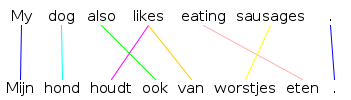
\includegraphics[scale=0.6]{alignment.png}
\caption{A one-to-many alignment of the English sentence `My dog also likes eating sausages.' and its translation `Mijn hond houdt ook van worstjes eten'.%schrijf welke tool is gebruikt
\cite{maillette2010visualizing}
}\label{fig:alignment}
\end{figure}

Alignments can be of several types, which will be of importance for the complexity of our algorithms. A summary can be found in table \ref{table:alignments}.


\begin{table}[!ht]
\begin{tabular}{|ll|}
\hline
one-to-one & $\forall x\forall y \big( (x,y)\!\in\!y \to \forall z \big( (z,y)\!\in\!a \to z\!=\!x \land (x,z) \!\in\! a \to z\!=\!y \big ) \big ) $\\
&\\
one-to many & $\forall x\forall y \big( (x,y)\!\in\!y \to \forall z \big( (z,y)\in a \to z\!=\!x \big) \big) $\\
&\\
many-to-one & $\forall x\forall y \big( (x,y)\!\in\!y \to \forall z \big( (x,z)\!\in\!a \to z\!=\!y \big) \big ) $\\
&\\
many-to-many & - \\
&\\
monotone & $\forall w \forall x\forall y \forall z \big ( \left ( (x,y)\in a \land (w,z)\in a \land x < w \right ) \to y < z \big )$\\
\hline
\end{tabular}
\caption{Alignment types, restrictions}
\label{table:alignments}
\end{table}

For the following definitions, we will introduce a change in notation. In our new notation, alignments are represented as extended permutations, in which numbers of the original sequence are allowed to appear more than once, or not at all. We will call such a representation a set-permutation. A set-permutation is defined as follows:

\begin{definition}[Set-permutation]
Given a source sentence $s = s_0 \ldots s_n$, its translation $t = t_0 \ldots t_m$, and an alignment $a$, let $a(i) = \{j~|~(i,j)\in a\}$ be the set with target positions that is linked to source position $i$. The set-permutation $\pi$ uniquely describing $a$ is defined as the ordered sequence of sets
$\langle a(0), \ldots, a(n) \rangle$
\end{definition}

The set-permutation $\pi = \langle\pi_0, ..., \pi_n\rangle$ describing the alignment depicted in Figure \ref{fig:alignment} would thus be $\langle \{0\}, \{1\}, \{3\}, \{2,4\}, \{6\}, \{5\}, \{7\}\rangle$. In the following definitions it is assumed that there are no unaligned target-words (thus for a sentence with $n$ words, $\bigcup_{i=0}^n \pi_i$ constitutes a contiguous sequence of numbers). The definitions can easily be extended to the case where there are unaligned target words, by only numbering the target positions that are aligned (effectively shifting the position numbers to the left whenever an unaligned word is found).

\subsubsection{Translation Units} To define a tree over an alignment, we need to have a notion of allowed sub sequences. For this, we use a definition analogous to the definitions of phrase pair used in the first phrase based models \citep{och2004alignment}. For this we will use the notion of span:

\begin{definition}[Span]
Given a sentence $s = s_1\ldots s_n$ with set-permutation $\pi$, a span $[i,j]$ denotes the subset $\pi_i\ldots pi_j\subseteq \pi$ corresponding to words $s_i\ldots s_j$
\end{definition}

A phrase pair is a pair of source and target spans $[i,j]$ and $[x,y]$, respectively, such that at least one word in $[i,j]$ is aligned to at least one word in $[x,y]$, and no words in $[i,j]$ are aligned to words outside $[x,y]$ and vice versa. The phrases consistent with the alignment are thus phrases whose translation is also a phrase. Translated in terms of a set-permutations $\pi$, we get the following definition for a translation unit:

\begin{definition}[Translation unit]
A span [$i,j$] representing contiguous sequence $s_i\ldots s_j$ of a source sentence whose alignment is represented by a set-permutation $\pi = \langle\pi_0 ,\ldots ,\pi_n\rangle$ is a possible translation unit iff the union $(\pi_i\cup \ldots \cup \pi_j)$ constitutes a contiguous range of integers, and for every integer $x \in (\pi_i\cup \ldots \cup\pi_j)$ holds that  $x \notin (\pi_0\cup \ldots \cup \pi_{j-1} \cup \pi_{i+1}\cup\ldots\cup \pi_n)$.
\end{definition}

The set of translation units consistent with the alignment in Figure \ref{fig:alignment} is thus: {[0,0], [1,1], [2,3], [4,4], [5,5], [0,1], [2,3], [4,5], [1,3], [0,4], [2,5], [0,5]}. In which [x,y] includes all words from position $x$ to position $y$. Note that the word 'like' is not a translation unit on its own, as it translates into two non-adjacent words in the Dutch target sentence. To cover such cases, we introduce `discontinuous translation units', that refer to any pair of source and target sequences that translate into each other (and only into each other), but are not contiguous. A subsequence of a `discontinuous translation unit' is an allowed part of the unit iff both its left and its right neighbour are not part of the unit.\\
The number of translation units in an alignment depends on the type of the alignment and is largest in case of a monotone alignment, that does not restrict the set of possible translation units at all. A completely monotone alignment of a sentence of $n$ words has $\frac{n\times n+1}{2}$ translation units. Note that unaligned words can cause exponential growth in the number of translation units.

\subsubsection{Alignment Trees} Given the set of translation units, we can define the set of structures according to which the sentence could have been compositionally translated. To define this set of structures, we firstly introduce the notion of a segmentation of a set-permutation.

\begin{definition}[Segmentation of a set-permutation]
Let $\pi = \langle \pi_0, \ldots,\pi_n\rangle$ be a set-permutation. A segmentation of $\pi$ is an ordered set of indices $B = \{j_0 = 0, j_1, \ldots ,j_{m-1},j_m = n+1\}$ that segments $\pi$ into $m$ adjacent, non-overlapping and contiguous segments such that for all $0\leq i < m$ holds that the subsequence $\pi_{j_i}\ldots\pi_{j_{i+1}-1}$ is either a translation unit or an allowed part of a discontinuous translation unit.
\end{definition}

For instance, a possible segmentation of our running example (recall: $\pi = \langle \{0\}, \{1\}, \{3\}, \{2,4\}, \{6\}, \{5\}, \{7\}\rangle$) would be $\{0,1, 2,4,7\}$, as it divides the sequence in allowed spans $[0,0]$, $[1,1]$, $[2,3]$ and $[4,6]$. We can now define the set of alignment trees:

\begin{definition}[Alignment tree]
Given a source sentence $s = s_0 \ldots s_n$ and the set of its translation units $U = \{u_1,\ldots,u_m\}$. An alignment tree is any tree $T$ satisfying the following four conditions:\begin{enumerate}
\item $[0,n]$ is the root of the tree
\item For the set $N = \{n~|~n$ is a node in $T\}$ holds: $N\supseteq \{[i,i]~|~0\leq i\leq n\}$
\item For every node $n\in N$ holds $U\cup \{[i,i]~|~0\leq i\leq n\}$ or $n$ is a word in the sentence
\item For every node $[i,j] \in N$ with children $[x_1,y_1]\ldots [x_n,y_n]$ holds: $x_k = y_{k-1}+1$ and $\{x_1,\ldots x_n, y_n+1\}$ is a segmentation of $[i,j]$
\end{enumerate}
\end{definition}

An alignment may have many different possible alignment trees. The number of alignment trees can be exponential in the length of the sentence, if no restriction is placed on the branching factor of the nodes. Every alignment can be assigned at least one structure (the completely flat one). A possible alignment tree for the alignment of the example can be found in Figure \ref{fig:alignment_tree}.

\begin{figure}
\Tree [.[0,6] [.[0,1] [.[0,0] my ] [.[1,1] dog ] ] [.[2,6] [.[2,4] [.[2,2] also ] [.[3,3] likes ] [.[4,4] eating ] ] [.[5,6] [.[5,5] eating ] [.[6,6] sausage ] ] ] ] ]
\caption{A possible alignment tree for the alignment of Figure \ref{fig:alignment} \label{fig:alignment_tree}}
\end{figure}

\subsubsection{Hierarchical Alignment Trees}

HATs, as defined in \cite{simaan2013hats}, are a strict subset of all alignment trees, in which all nodes have a minimal branching factor:

\begin{definition}
A HAT is an alignment tree in which the fourth criterion is replaced by the following:
\begin{enumerate}
\item[4.] For every node $[i,j] \in N$ with children $[x_1,y_1]\ldots [x_n,y_n]$ holds: $x_k = y_{k-1}+1$ and $\{x_1,\ldots x_n, y_n\}$ is a segmentation $B$ of $[i,j]$ such that for all other segmentations $B'$ of $[i,j]$ holds that $|B'|\geq |B|$ %Dit moet ook net iets anders)
\end{enumerate}
\end{definition}

Furthermore, the nodes of the HATs are decorated with ITG-like operators, that specify how the target-side HAT can be constructed. An example of a HAT can be found in Figure \ref{fig:hat}.

\begin{figure}
\caption{Example HAT, anders}\label{fig:hat}
\end{figure}

A HAT with operators uniquely determines a word-alignment, in a maximally recursive fashion. The latter is desirable, not only for practical reasons - it reduces the number of rules significantly, but also because it maximises the probability that we can generalise to new data. \cite{simaan2013hats} provide empirical data, some of which were discussed in the previous section, describing what percentage of alignments can be explained by constrained versions of HATs. 

\subsubsection{The Power of HATs}

If no constraints are imposed, HATs can describe \textit{any} word alignment, which makes them a very powerful tool. Its power and generality with respect to our goal can be captured in two properties, that we will elaborate on in the following two paragraphs.

\paragraph{Non isomorphic source and target structures.} As the operators on the nodes of the HATs are set-permutations on their own, they can describe the existence of nodes in the target side structure that do not match precisly one source side node. This allows for a natural description of structures that cannot be described in the SCFG framework. An example is shown in \ref{fig:nepas} in which a HAT for the translation of `I don't smoke' into `Je ne fume pas', which is generally problematic for SCFG's, is depicted.

\begin{figure}
\caption{}\label{fig:nepas}
\end{figure}

\paragraph{HATs describe a non-bijective mapping.} From the non-isomorphism follows (anders) that the mapping between nodes in HATs is non-bijective, but the mapping between complete HATs is not necessarily bijective either, if the HATs are seen as (potentially labelled) structures.\footnote{Maybe further explain in this footnote?} To illustrate this, consider the following example of translation from English to Danish. The English sentences `I give you flowers', and `I give flowers to you' can both be translated into to the Danish `jeg giver dig blomster' (although `jeg giver blomster til dig' would be a more appropriate translation for the second sentence, as it meets the criterion of being literal). In Figure \ref{fig:nonbij}, we see that the two linguistically plausible structures for the English sentences map to the same structure for the Danish sentence. As the two Danish sentences are identical, we may assume that if someone would assign labels to the nodes, the labels assigned to both trees would be identical as well, and hence we have established that the mapping between labelled structures is at least many-to-one. As the same argument holds in the other direction (i.e., both `jeg giver blomster til dig' and `Jeg giver dig blomster' can be found in the corpus as translation of `I give you flowers'), from which we can conclude that the mapping between HATs can be in principle many-to-many. Clearly, when we take into account the operators as labels, the mapping is one-to-one. 

\begin{figure}
\caption{Non bijective mapping}\label{fig:nonbij}
\end{figure}

In translation from English to Danish, this example is slightly artificial, as we normally require translations to be literal (anders). Nevertheless, examples like this might occur in corpora, and it is nice to see that HATs can in principle even account for small amounts of freedom during translation. Furthermore, examples like this might also occur in translation between languages that differ in the level of generality in expressing certain meanings. For instance, such a difference arises when the English word `go' is translated into Russian, where it is required to specify whether you walked (\textcyr{idti}) or used a vehicle (\textcyr{ehat\char126}), as a general verb that describes going from A to B does not exist in Russian.

\subsection{Experiments}

Before describing our experiment, (anders) recall that the main aim of this paper is investigating the assumptions underpinning compositional translation. In particular, we want to see if it is possible to find recursive structures of sentences and a systematic mapping between them. The HATs are a very powerful tool for doing so, as they can describe any translation from source to target side. However, the mapping from word-alignments to HATs is a one-to-many mapping: a HAT uniquely describes a word-alignment, but a word alignment is often described by many HATs. To confirm that compositional translation is a reasonable strategy, we need something more: a way of producing a single HAT for a word alignment that is consistent over all sentences.\footnote{Two remarks are needed to refine this statement. Firstly we assume that a sentence has only one meaning, which rules out ambiguity cases. If a sentence has multiple meanings, different HATs might correspond to these meanings. This thesis considers such ambiguity aspects a separate problem, which is not taken into account here at all. Secondly, it is mainly theoretical that we want to find \textit{one} HAT per alignment. This is not to say, that in practice it might not be more desirable to generate multiple HATs per sentence over which a probability distribution can be defined. (anders)} In this thesis we are concerned with finding such a consistent set of HATs for a corpus. There can be exponentially many HATs per sentence (compute how many?), and statistically learning this set without any external reference seems out of reach. Given that the nature of translation is preservation of the semantic content of a sentence, it seems reasonable to assume that the structural representation of a translation is semantically motivated. We will therefore use dependency parses \citep{schubert1987metataxis}, which specify the predicate argument structure of a sentence as perceived by humans, to guide us in our search. Hereby, we implicitly address the question: are predicate argument structures preserved during translation. As in many previous empirical investigations, we will only focus on source side structures (at first), without worrying about the consistency of the target side structures they are mapped to, implying that we will not consider the node operators. If no consistent source side structures can be found, there is no hope for finding consistent pairs of structures, rendering compositional translation a limited strategy.

\subsubsection{Experiment 1}

%Maybe give the definition of HATs and dependency parses here.

The predicate argument relations in a dependency tree tell us exactly how the sentence is composed: we can infer which are the smaller parts of the sentence and how they are combined to obtain the complete sentence. Consider for instance the dependency tree of the sentence "My dog also likes eating sausage" (Figure \ref{fig:deptree1}).

\begin{figure}[!h]\label{fig:deptree1}
\centering
\begin{dependency}[theme=simple]%[hide label]
\begin{deptext}[column sep=.5cm, row sep=.1ex]
%PRP\$ \& NN \& RB \&[.5cm] VBZ \& VBG \& NN \\
My \& dog \& also \& likes \& eating \& sausage \\
\end{deptext}
\deproot{4}{}
\depedge{2}{1}{poss}
\depedge{4}{2}{nsubj}
\depedge{4}{3}{xvmod}
\depedge{4}{5}{xcomp}
\depedge{5}{6}{dobj}
\end{dependency}
\caption{Stanford Dependency Tree}
\end{figure}

The dependency tree tells us that 'likes' is the head word of the sentence, and that the sentence is composed of 4 parts: the head `likes', its modifier `also', its noun subject whose head is `dog' and the open clausal complement whose head is `eating'. The complement and subject are further divisible in `My' and `dog', and `eating' and `sausage', respectively. Intuitively, we can check for every relation in the dependency parse whether this relation exists in a HAT by checking if the word and its depending subtrees are siblings in the HAT. We will then say that such a relation is respected by the HAT, as is defined in Definition \ref{def:depHAT}.



\begin{definition}\label{def:depHAT}
Let $s = w_1 w_2 \dots w_n$ be a sentence, and $D = \{ (i,j) |$ there is a dependency arrow from word $w_i$ to word $w_j \}$ a set of dependencies describing a dependency tree for $s$. Let span($j$) be the range $[m,n]$ in which $m$ and $n$ are the maximum and minimum position that can be reached from $w_j$ by following the directed dependency arrows, respectively. A dependency relation $(i,j)$ is said to be respected by an alignment tree $T$ over $s$ if and only if there is a node in $T$ of which both $[i,i]$ and span($j$) are children.
\end{definition}

In a first experiment, we will search for the HAT that respects the highest percentage of the dependency relations prescribed by the dependency parse. Note that relations within phrasal translations will always be consistent with the HATs, as words that are part of a phrasal translation are necessarily siblings. Phrasal translations do thus not demand a special treatment, as they are naturally covered.

\subsubsection{Follow-up Experiments}


In the best case, we can find a HAT for every sentence in which all dependency relations are preserved. However, we suspect that we will not achieve perfect scores. If so, we will further investigate if improvement on the result is possible. We have distinguished five reasons that could lower the score:

\begin{enumerate}
\item The translation is erroneous, or non literal;
\item The dependency parse is erroneous;
\item The alignment is erroneous;
\item The structure of HATs and dependency parses does not agree;
\item The sentence cannot be compositionally translated.
\end{enumerate}

Empirical research like this, using translation corpora, hinge on the assumption that the datasets we use are representative for the phenomena we are investigating, and are error-free. Unfortunately, this is often not the case. Dependency parsers are not perfect, the translations in our corpora are not always as literal as we would want them to be, and automatic alignments often contain many incorrect alignment links. Although these factors can play an important role, there is not much that we can do about it: we cannot instruct interpreters of the government to follow a protocol specifically designed for our needs\footnote{Or can we...}, and we do not have the manpower to filter our corpora or produce manual alignments for corpora of a reasonable size. Even in empirical research, testing the influence of these factors often boils down to manually checking the data. We will consider the influence of the alignments by running the same experiments on manually aligned datasets. Regarding the first two causes, we might perform a manual analysis on a small subset of our data, but not before we have investigated the fourth case: a discrepancy between the dependency parses and the HATs. We consider this likely to be an issue as we have forced our trees to be maximally recursive. Maximal recursivity is very useful for computational purposes, but it is likely not the structure that corresponds to human intuitions. We will illustrate this with two examples.\\
Firstly, consider the sentence `I give you flowers', which contains one predicate (`give') with three arguments (the subject `I', the object `flowers' and the indirect object `you'). Its Dutch translation `Ik geef jou bloemen' has exactly the same predicate argument structure \textit{and} word-order, whereby the branching factor in any of its HATs will not exceed two. However, a maximum score can only be obtained by a tree in which `I', `give', `you', and `flowers' are siblings, whose mother will have a branching factor of (at least) four. Even though the translation of this sentence seems perfectly compositional, no HAT will thus obtain the maximum score, because the dependency structure is not minimally branching.\\
A second example, that is more related to translational divergence, arises when two arguments are translated into one (which happens, e.g., when arguments are translated as pre- or suffixes, when verbs do not require a subject or when spaces are emitted). Consider for instance the sentence 'Can you give me the salt' and its Italian translation 'puoi passarmi il sale'. Once again, the predicate-argument structure of the sentence is well preserved. However, the dependency parse prescribes that `the salt', `can' and `you' should be siblings of `give', which will be the case in none of the HATs over $\{\{0\},\{0\},\{1\},\{1\},\{2\},\{3\}\}$, as `give' and `me' are together translated into `passarmi', and `can you' into `puoi'.\\
%Anders
Both cases could be solved when considering dependency motivated labels similar to the ones defined in \cite{zollmann2006syntax} that represent compound categories, which we will do in a second experiment (e.g., `give you flowers' could be seen as a sentence missing a subject to the left (subj\textbackslash S) and `I give' as a combination of a subject and a verb (subj+verb)). We will investigate these new labels by determining how often they are translation units in the alignments. Subsequently, we will rescore the HATs with the new labels, slightly adapting the scoring metric. Instead of looking at sibling relations, we will consider how many of the nodes in the HAT can be labelled using a label from our new label set. A HAT will receive a score corresponding to the percentage of its nodes that could be labelled and thus receives a maximum score if all of its nodes could be labelled. Note that this introduces a slight bias towards trees with more nodes: a tree with 10 nodes of which one is unlabelled receives a higher score than a tree with 9 nodes of which one is unlabelled.\\
Appropriate einde van hoofdstuk%Explain why we do not think this is problematic?




%%%%%%%%%%%%%%%%%%%%%%%%%%%%%%%%%%%%%%%%%%%%%%%%%%%%%%%%%%%%%%%%%%%%%%%%%%%%%%%%%%%%%%%%%%%%%%%%%%%%%%%%%%%%%%%%%%%%%%%%%%%%%%%%%%%%%%%%%%%%%%%%%%%%%%
%%%%%%%%%%%%%%%%%%%%%%%%%%%%%%%%%%%%%%%%%%%%%%%%%%%%%%%%%%%%%%%%%%%%%%%%%%%%%%%%%%%%%%%%%%%%%%%%%%%%%%%%%%%%%%%%%%%%%%%%%%%%%%%%%%%%%%%%%%%%%%%%%%%%%%
% EXPERIMENTS
%
% Describing the experiments and their results
%


\chapter{Experiments and Results}

%Other introduction?
In this chapter we will present our empirical results, and give a precise description of the procedures used to obtain them. Documentation of the code can be found in Appendix \ref{appendix:impl}.\\

\section{General Setup}



In all our experiments, we search for the HAT that is most consistent with a set of relations that are abstracted from a set of basic dependencies of the (English) sentence, generated by the Stanford Dependency parser \cite{de2006generating}. Details on this set of relations can be found in the sections dedicated to the different experiments.\\

\subsection{Procedure and Algorithms}

We searched through the HATs by generating a grammar for every alignment that uniquely generated the HAT forest for that alignment, and manipulating the probabilities of the rules to find the best HAT using an off-the-shelve Viterbi parser \citep{bird2009natural}. This grammar was generated by creating a graph representation of the alignment, and searching for the shortest path between the endpoints of all allowed translation units, as is depicted in \ref{alg:grammar}. Auxiliary algorithms \ref{alg:shortest paths} and \ref{alg:phrasepairs} describe the how the shortest paths were found and how the translation units were identified, respectively.

\begin{algorithm}
\caption{Grammar generation}\label{alg:grammar}
\begin{algorithmic}
\STATE \textbf{Input:} A sentence $s = w_1\ldots w_n$ and a string representation of alignment $a$
\STATE \textbf{Output:} A grammar uniquely generating the HAT forest
\STATE %nothing
\STATE alignment = set\_repr($a$) \hfill \# Represent alignment as a set
\STATE U = translation\_units($a$) \hfill \# Find translation units of $a$ 
%DIT MOET ANDERS!!!
\STATE \textit{\# Create a graph representation of the alignment}
\STATE $V = \{\}$
\FOR{$i\in\{0,n\}$}
	\STATE $V$ $\leftarrow$ $V\cup v_i$
\ENDFOR
\STATE $E=\{\}$
\FOR{$(i,j)\in U$}
	\STATE $E$ $\leftarrow E\cup (i$-$1,j)$
\ENDFOR
\STATE \textit{\# Compute rules for every translation unit}
\STATE rules = $\emptyset$
\FOR{$(i,j)\in U$}
	\IF{$i+1 = j$}
		\STATE new\_rule = $(i,j) \leftarrow w_j$)
		\STATE rules $\leftarrow$ rules $\cup$ new\_rule 
	\ELSE
		\FOR{path $(i,r_1,\ldots,r_m,j)$ $\in$ shortest\_paths$(i,j)$}
			\STATE new\_rule = $(i,j \leftarrow (i,r_1) (r_1, r_2) \ldots (r_m j)$
			\STATE rules $\leftarrow$ rules $\cup$ new\_rule
		\ENDFOR
	\ENDIF
\ENDFOR
\end{algorithmic}
\end{algorithm}

Algorithm \ref{alg:shortest paths}, which is similar to Dijkstra's shortest path algorithm \citep{dijkstra1959note}, was used to compute the shortest paths from $i$ to $j$.

\begin{algorithm}
\caption{Shortest Paths}\label{alg:shortest paths}
\begin{algorithmic}
\STATE \textbf{Input:} A graph $G = (V,E)$ describing an alignment and two vertices $i$ and $j$ for which $(i,j)\in E$ is true.
\STATE \textbf{Output:} All non-trivial shortest paths from $i$ to $j$
\STATE \textit{\#Initialization}
\STATE visited = $\emptyset$, depth = $0$, paths = $\{j\}$
\STATE $\forall n\in\mathbb{N}:$ reachable(n) = $\emptyset$; reachable($0$) = $\{j\}$
\STATE depth\_finished = False
\STATE \textit{\# Start backwards search through graph}
\WHILE{not depth\_finished or $i\notin$ visited}
	\WHILE{reachable(depth) $\neq\emptyset$}
		\STATE depth\_finished $\leftarrow$ False
		\STATE current\_node $\leftarrow N$ an arbitrary element $v$ from reachable(depth)
		\STATE reachable(depth) $\leftarrow$ reachable(depth) $-$ $\{$current\_node$\}$
		\FOR{ ($l$,current\_node) $\in E$}
			\IF{$l\notin $visited $\cup$ reachable(depth) \AND depth $\neq 0$}
				\STATE reachable(depth+1) $\leftarrow$ reachable(depth+1) $\cup$ $\{l\}$
				\FOR{path (current\_node,\ldots, $j) \in$ paths}
					\STATE path $\leftarrow$ ($l$,current\_node,\ldots, $j)$
				\ENDFOR
			\ENDIF
		\STATE visited $\leftarrow$ visited $\cup$ $\{l\}$
		\ENDFOR
	\STATE depth\_finished $\leftarrow$ True
	\STATE depth $\leftarrow$ depth+1
	\ENDWHILE
\ENDWHILE
\STATE \textbf{Return} paths
\end{algorithmic}
\end{algorithm}

The translation units are found using an algorithm similar to the one presented in \cite{chiang2005hierarchical} (is it this one??), which is described in Algorithm \ref{alg:phrasepairs}.

\begin{algorithm}
\caption{Finding translation Units}\label{alg:phrasepairs}
\begin{algorithmic}
\STATE \textbf{Input:} an alignment graph $G = (V,E)$
\STATE \textbf{Output:} all allowed translation units.
\end{algorithmic}
\end{algorithm}


\subsection{Data}

Describe corpora, which sections are used and how they were aligned.

\begin{table};!h]
\begin{tabular}{llllll}
Language & Corpus & & Section & Aligned\\
\hline
English - Dutch & Europarl & & automatic \\
English - French & Europarl & automatic \\
English - German & Europarl & automatic \\
English - Chinese & & & automatic \\
English- French & Hansard & & manual\\
\end{tabular}
\caption{Datasets}\label{tab:datasets}
\end{table}

We parsed the English side of the corpus with the Stanford dependency parser \citep{de2008stanford} using newlines as delimitation, to obtain basic typed dependencies of the sentences. Note that punctuation is thus not taken into account.

\subsection{Shared Notions}



\section{Experiment 1}

As mentioned before, we will test the HATs of an alignment for consistency with a set of relations abstracted from the dependency parse of the corresponding sentence. In Experiment 1, this will be done in the most elementary way of doing so, which we will explain in the following subsection.
%Explain what comes after

\subsection{Motivation}

The predicate argument relations in a dependency tree tell us exactly how the sentence is composed: we can infer which are the smaller parts of the sentence and how they are combined to obtain the complete sentence. Consider or instance the dependency tree of the sentence `My dog also likes eating sausage' (\ref{fig:deptree}).

\begin{figure}[!h]\label{fig:deptree}
\centering
\begin{dependency}[theme=simple]%[hide label]
\begin{deptext}[column sep=.5cm, row sep=.1ex]
%PRP\$ \& NN \& RB \&[.5cm] VBZ \& VBG \& NN \\
My \& dog \& also \& likes \& eating \& sausage \\
\end{deptext}
\deproot{4}{}
\depedge{2}{1}{poss}
\depedge{4}{2}{nsubj}
\depedge{4}{3}{xvmod}
\depedge{4}{5}{xcomp}
\depedge{5}{6}{dobj}
\end{dependency}
\caption{Stanford Dependency Tree}
\end{figure}

The dependency tree shows that `likes' is the head word of the sentence, and that the sentence is composed of four parts: the head `likes', its modifier `also', its noun subject whose head is `dog' and the open clausal complement whose head is `eating'. The complement and subject are further divisible in `My' and `dog', and `eating' and `sausage', respectively. Intuitively, we can check for every relation in the dependency parse whether this relation exists in a HAT by checking if the word and its depending subtrees are siblings in the HAT. Experiment 1 is based upon this definition.

\subsection{Relations}

We will say that a dependency relation from word $i$ to word $j$ is respected by a HAT if the head $i$ is siblings with the phrases headed by $j$, which is formally defined in \ref{def:respHAT}

\begin{definition}\label{def:respHAT}
Let $s = w_1 w_2 \dots w_n$ be a sentence, and $D = \{ (i,j) |$ there is a dependency arrow from word $w_i$ to word $w_j \}$ a set of dependencies describing a dependency tree for $s$. Let span($j$) be the range $[m,n]$ in which $m$ and $n$ are the maximum and minimum position that can be reached from $w_j$ by following the directed dependency arrows, respectively. A dependency relation $(i,j)$ is said to be respected by an alignment tree $T$ over $s$ if and only if there is a node in $T$ of which both $[i,i]$ and span($j$) are children.
\end{definition}

In Experiment 1, we will search for the HAT in which most of these relations are respected, as defined in \ref{metric:m1}.

\begin{metric}\label{metric:m1}
Let $s = w_1 w_2 \dots w_n$ be a sentence, and $D = \{ (i,j) |$ there is a dependency arrow from word $w_i$ to word $w_j \}$ a set of dependencies describing a dependency tree for $s$. Let $D' = \{ (i,\textrm{span}(j))$ $|$ $D(i,j) \land 1 \leq i,j \leq n \}$ be the set $D$ in which each dependent $w$ is replaced by its span $[i,j]$, with $i$ and $j$ the maximum and minimum position, respectively, that can be reached from $w$ by following the directed dependency arrows. Let $H$ be an alignment tree for $s$. The consistency of $H$ with $D$ is now defined as the score of its highest node $N$::

$$
E(N_a,D) = \sum_{c\in C_{N_a}} E(c,D)+ \sum_{c_1\in C_{N_a}} \sum_{c_2\in C_{N_a}} B(c_1,c_2)
$$

\noindent With base case $E(N,D) = 0$, $B(c_1,c_2) = 1$ iff  $(c_1,c_2)\in D'$, and $C_N$ the set of child nodes of $N$.
\end{metric}

Note that this score should be normalized after the procedure by dividing by $|D'|$. As $|D'|$ is not dependent on the tree, this does not complicate the search for the best HAT.

\subsection{Search}

The grammar productions $r$ were found as described before, and were assigned weights according to the number of relatios $n$ they made true: $r = 2^n$. These weights do not constitute a probability model (as indicated by the fact the `probabilities' can be higher than $1$), but are meant to guide the search. A proof of soundness of this procedure is given below.

\begin{proof}[Soundness of Procedure]
\label{proof:s1}
to proof: score(N1) $>$ score(N2) iff p(N1) $>$ p(N2)
\end{proof}

An external parser was used \citep{bird2009natural} to parse the sentence into the best HAT.

\subsection{Results}

The results of Experiment 1 can be found in table \ref{tab:scores1}

\begin{table}[!h]
\centering
\begin{tabular}{l|ccc}
& \multicolumn{3}{c}{Multi-column}\\
Language pair & |s| < 10 & |s| < 20 & |s| < 40\\
\hline
English-Dutch & 0.450 & 0.408 & 0.390 \\
English-French & 0.431 & 0.412 & 0399 \\
English-German & 0.423 & 0.395 & 0.376 \\
English-Chinese & 0.410 & 0.382 & 0.361\\
\end{tabular}
\caption{Results Experiment 1, automatic alignments}\label{tab:scores1}
\end{table}

%table with which results were respected?

\section{Experiment 2}

\subsection{Motivation}

Experiment 1 showed that HATs are not very consistent with dependency parses: on average not even half of the relations from the dependency parse of a sentence were respected in a maximally recursive alignment tree. However, drawing the conclusion that dependency syntax is thus useless for SMT without considering other options would be rather hasty. We have identified five reasons that possibly could have lead to a low score for an alignment:

\begin{enumerate}
\item The translation is erroneous or not as literal as possible;
\item The dependency parse is erroneous;
\item The alignment is erroneous;
\item The structure of HATs and dependency parses does not agree;
\item The sentence cannot be compositionally translated
\end{enumerate}

Empirical research using translation corpora hinges on the assumption that the datasets that are used are error-free and representative for the phenomena that are investigated. Although this is often not the case - dependency parses are not perfect, the translations in our corpora are not always as literal as we would want them to be, and automatic alignments often contain many incorrect alignment links - for the moment we will stick to this assumption. Although these factors can play an important role, there is not much that we can do about it: we cannot instrut interpreters of the government to follow a protocol specifically designed for our needs, and we do not have the manpower to filter our corpora or produce manual alignments for corpora of a reasonable size. Even in empirical research, testing the influence of these factors often boils down to manually checking the data, which we will only do after having considered other options.\\
In Experiment 2 we investigate the discrepancy between dependency parses and HATs (cause 4), which we consider likeli to be an issue, as we have forced our trees to be maximally recursive. Maximal recursivity is very useful for computational purposes and generalization (ref?), but it is likely not the structure that corresponds to human intuitions. We will illustrate this with two examples.\\ 
Firstly, consider the sentence `I give you flowers', which contains one predicate (`give') with three arguments (the subject `I', the object `flowers' and the indirect object `you'). Its Dutch translation `Ik geef jou bloemen' has exactly the same predicate argument structure \textit{and} word-order, whereby the branching factor in any of its HATs will not exceed two. However, a maximum score can only be obtained by a tree in which `I', `give', `you', and `flowers' are siblings, whose mother will have a branching factor of (at least) four. Even though the translation of this sentence seems perfectly compositional, no HAT will thus obtain the maximum score, because the dependency structure is not minimally branching.\\
A second example, that is more related to translational divergence, arises when two arguments are translated into one (which happens, e.g., when arguments are translated as pre- or suffixes, when verbs do not require a subject or when spaces are emitted). Consider for instance the sentence 'Can you give me the salt' and its Italian translation 'puoi passarmi il sale'. Once again, the predicate-argument structure of the sentence is well preserved. However, the dependency parse prescribes that `the salt', `can' and `you' should be siblings of `give', which will be the case in none of the HATs over $\{\{0\},\{0\},\{1\},\{1\},\{2\},\{3\}\}$, as `give' and `me' are together translated into `passarmi', and `can you' into `puoi'.\\










% END OF RESULTS
%%%%%%%%%%%%%%%%%%%%%%%%%%%%%%%%%%%%%%%%%%%%%%%%%%%%%%%%%%%%%%%%%%%%%%%%%%%%%%%%%%%%%%%%%%%%%%%%%%%%%%%%%%%%%%%%%%%%%%%%%%%%%%%%%%%%%%%%%%%%%%%%%%%%%%
%%%%%%%%%%%%%%%%%%%%%%%%%%%%%%%%%%%%%%%%%%%%%%%%%%%%%%%%%%%%%%%%%%%%%%%%%%%%%%%%%%%%%%%%%%%%%%%%%%%%%%%%%%%%%%%%%%%%%%%%%%%%%%%%%%%%%%%%%%%%%%%%%%%%%%





%%%%%%%%%%%%%%%%%%%%%%%%%%%%%%%%%%%%%%%%%%%%%%%%%%%%%%%%%%%%%%%%%%%%%%%%%%%%%%%%%%%%%%%%%%%%%%%%%%%%%%%%%%%%%%%%%%%%%%%%%%%%%%%%%%%%%%%%%%%%%%%%%%%%%%
%%%%%%%%%%%%%%%%%%%%%%%%%%%%%%%%%%%%%%%%%%%%%%%%%%%%%%%%%%%%%%%%%%%%%%%%%%%%%%%%%%%%%%%%%%%%%%%%%%%%%%%%%%%%%%%%%%%%%%%%%%%%%%%%%%%%%%%%%%%%%%%%%%%%%%
% DISCUSSION
%
%

\chapter{Discussion and Future Work}

short summary of findings and what they mean

%future work: source reordering, treebank to learn translation structure
% promising for further models: monolingual parsing and learning reordering operators


%
% 
% END OF DISCUSSION
%%%%%%%%%%%%%%%%%%%%%%%%%%%%%%%%%%%%%%%%%%%%%%%%%%%%%%%%%%%%%%%%%%%%%%%%%%%%%%%%%%%%%%%%%%%%%%%%%%%%%%%%%%%%%%%%%%%%%%%%%%%%%%%%%%%%%%%%%%%%%%%%%%%%%%
%%%%%%%%%%%%%%%%%%%%%%%%%%%%%%%%%%%%%%%%%%%%%%%%%%%%%%%%%%%%%%%%%%%%%%%%%%%%%%%%%%%%%%%%%%%%%%%%%%%%%%%%%%%%%%%%%%%%%%%%%%%%%%%%%%%%%%%%%%%%%%%%%%%%%%




%%%%%%%%%%%%%%%%%%%%%%%%%%%%%%%%%%%%%%%%%%%%%%%%%%%%%%%%%%%%%%%%%%%%%%%%%%%%%%%%%%%%%%%%%%%%%%%%%%%%%%%%%%%%%%%%%%%%%%%%%%%%%%%%%%%%%%%%%%%%%%%%%%%%%%
%%%%%%%%%%%%%%%%%%%%%%%%%%%%%%%%%%%%%%%%%%%%%%%%%%%%%%%%%%%%%%%%%%%%%%%%%%%%%%%%%%%%%%%%%%%%%%%%%%%%%%%%%%%%%%%%%%%%%%%%%%%%%%%%%%%%%%%%%%%%%%%%%%%%%%
% CONCLUSION
%
%

\chapter{Conclusion}

%
%
% END OF CONCLUSION
%%%%%%%%%%%%%%%%%%%%%%%%%%%%%%%%%%%%%%%%%%%%%%%%%%%%%%%%%%%%%%%%%%%%%%%%%%%%%%%%%%%%%%%%%%%%%%%%%%%%%%%%%%%%%%%%%%%%%%%%%%%%%%%%%%%%%%%%%%%%%%%%%%%%%%
%%%%%%%%%%%%%%%%%%%%%%%%%%%%%%%%%%%%%%%%%%%%%%%%%%%%%%%%%%%%%%%%%%%%%%%%%%%%%%%%%%%%%%%%%%%%%%%%%%%%%%%%%%%%%%%%%%%%%%%%%%%%%%%%%%%%%%%%%%%%%%%%%%%%%%



%%%%%%%%%%%%%%%%%%%%%%%%%%%%%%%%%%%%%%%%%%%%%%%%%%%%%%%%%%%%%%%%%%%%%%%%%%%%%%%%%%%%%%%%%%%%%%%%%%%%%%%%%%%%%%%%%%%%%%%%%%%%%%%%%%%%%%%%%%%%%%%%%%%%%%
%%%%%%%%%%%%%%%%%%%%%%%%%%%%%%%%%%%%%%%%%%%%%%%%%%%%%%%%%%%%%%%%%%%%%%%%%%%%%%%%%%%%%%%%%%%%%%%%%%%%%%%%%%%%%%%%%%%%%%%%%%%%%%%%%%%%%%%%%%%%%%%%%%%%%%
% APPENDIX IMPLEMENTATION
%
%

\appendix
\chapter{Implementation}
\label{appendix:impl}

NLTK toolkit: \cite{bird2009natural}\\
Stanford Dependency Parser: \cite{de2008stanford}(?)

%
%
% END OF APPENDIX IMPLEMENTATION
%%%%%%%%%%%%%%%%%%%%%%%%%%%%%%%%%%%%%%%%%%%%%%%%%%%%%%%%%%%%%%%%%%%%%%%%%%%%%%%%%%%%%%%%%%%%%%%%%%%%%%%%%%%%%%%%%%%%%%%%%%%%%%%%%%%%%%%%%%%%%%%%%%%%%%
%%%%%%%%%%%%%%%%%%%%%%%%%%%%%%%%%%%%%%%%%%%%%%%%%%%%%%%%%%%%%%%%%%%%%%%%%%%%%%%%%%%%%%%%%%%%%%%%%%%%%%%%%%%%%%%%%%%%%%%%%%%%%%%%%%%%%%%%%%%%%%%%%%%%%%



%%%%%%%%%%%%%%%%%%%%%%%%%%%%%%%%%%%%%%%%%%%%%%%%%%%%%%%%%%%%%%%%%%%%%%%%%%%%%%%%%%%%%%%%%%%%%%%%%%%%%%%%%%%%%%%%%%%%%%%%%%%%%%%%%%%%%%%%%%%%%%%%%%%%%%
%%%%%%%%%%%%%%%%%%%%%%%%%%%%%%%%%%%%%%%%%%%%%%%%%%%%%%%%%%%%%%%%%%%%%%%%%%%%%%%%%%%%%%%%%%%%%%%%%%%%%%%%%%%%%%%%%%%%%%%%%%%%%%%%%%%%%%%%%%%%%%%%%%%%%%
% APPENDIX EVALUATION METRICS
%
%

\chapter{Metrics}
\label{appendix:metric}

\section{Notation}

Firstly, we will present some notation that is shared along the different metrics.

\begin{notion}
$T_d$ will refer to a dependency tree of a sentence $s = w_1 \dots w_n$, formed by a set of dependencies $D = \{ (i,j) |$ there is a dependency arrow from word $w_i$ to word $w_j \}$.
\end{notion}

\begin{notion}
If $T_d$ is a dependency tree for $s$, $w$ is a word in $s$ and $i$ and $j$ are the maximum and minimum positions, respectively, that can be reached from $w$ by following the directed dependency arrows. Then span($w$) = $[i,j]$.
\end{notion}

\begin{notion}
$T_a$ will be used to refer to an alignment tree of a sentence $s = w_1 \dots w_n$. The label $i-j$ will refer to the node that dominates span $[i,j]$. The highest node of $T_a$ will be denoted with $N_{T_a}$
\end{notion}

\begin{notion}
Let $T_d$ be a dependency tree with dependencies $D$, Then $D' = \{ (i,\textrm{span}(j))$ $|$ $D(i,j) \land 1 \leq i,j \leq n \}$ is the set in which each dependent is replaced by its span.
\end{notion}

\begin{notion}
If $N$ is a node in a tree $T_a$, $C_N$ denotes the set of child constituents of this node. If node $N$ dominates words $i$ to $j$ in $s$, then $dom(N)= [i,j]$
\end{notion}

\section{Metric 1}

\begin{metric}\label{m1}
Let $s = w_1 w_2 \dots w_n$ be a sentence, and $T_d$ and $T_a$ its dependency tree and an alignment tree, respectively. The score of $T_a$ is defined as the score of its highest node $N_{a}$:

$$
E(N_a,D) = \sum_{c\in C_{N_a}} E(c,D)+ \sum_{c_1\in C_{N_a}} \sum_{c_2\in C_{N_a}} B(c_1,c_2)
$$

\noindent With base case $E(N,D) = 0$ and $B(c_1,c_2) = 1$ iff  $(c_1,c_2)\in D'$. Dividing the resulting score by $|D'|$ will result in a normalized score.
\end{metric}

\noindent  Note if this definition is strictly followed more than half of the sibling checks is redundant, an algorithm computing the score of a tree would not have to perform them all.

\section{Metric 2}

\begin{metric}\label{m2}
Let $s = w_1 w_2 \dots w_n$ be a sentence, and $T_d$ and $T_a$ its dependency tree and an alignment tree, respectively. The score of $T_a$ is defined as the score of its highest node $N_{a}$:

$$
E(N_a,D) = \sum_{c\in C_{N_a}} E(c,D)+ \sum_{c_1\in C_{N_a}} \sum_{c_2\in C_{N_a}} B(c_1,c_2)
$$

\noindent With base case $E(N,D) = 0$ and $B(c_1,c_2) = 1$ iff  $|dom(c_2)| > 1 \land (c_1,c_2)\in D'$ the part of the sentence covered by $c_2$. Dividing the resulting score by $|D'|$ will result in a normalized score.
\end{metric}

Note that normalizing the score will sometimes result in zero division for shorter sentences whose dependency parses display no compositional structure, in this cases we will define the score of the sentence to be 0.


\subsection{Metric 1}


\subsection{Metric 2}

Explain that metric 1 reflects the similarity with the dependency parse, rather than giving a reasonable measure of compositionality. Explain why this is, that a part of the score can trivially be reached by just making a flat tree. Explain how to fix this. Explain that evaluation metric 2 won't alter the ordering of the trees, just their scores.
Explain that metric 2 thus just differs in the set of relations it considers: instead of considering all relations from the dependency parse, it only considers the relations that reflect compositionality, which captures the intuition that completely flat trees should be assigned a 0 score. Note that this means that this therefore does not alter the ranking of the trees set by metric 1, it just alters the scores associated with the trees.








%%%%%%%%%%%%%%%%%%%%%%%%%%%%%%%%%%%%%%%%%%%%%%%%%%%%%%%%%%%%%%%%%%%%%%%%%%%%%%%%%%%%%%%%%%%%%%%%%%%%%%%%%%%%%%%%%%%%%%%%%%%%%%%%%%%%%%%%%%%%%%%%%%%%%%
%%%%%%%%%%%%%%%%%%%%%%%%%%%%%%%%%%%%%%%%%%%%%%%%%%%%%%%%%%%%%%%%%%%%%%%%%%%%%%%%%%%%%%%%%%%%%%%%%%%%%%%%%%%%%%%%%%%%%%%%%%%%%%%%%%%%%%%%%%%%%%%%%%%%%%

%THINGS I SHOULDN'T FORGET TO MENTION!

% zeg iets over dat we op deze manier nicely omgaan met phrasal translations

% put statistics about the data, the dependency parses, everything

% ook wat analyses over complexiteit e.d. max grootte van de grammatica's dat soort zaken

% niet zo tevreden over hoe dependency grammars met conjunction omgaan, collapsed dependencies doen dit wel beter trouwens, misschien moet ik daar nog eens naar kijken. Collapsed dependencies doen soms ook al wat werk met idiom (zie tabel 3)

%Geen enkel vertaalsysteem vertaalt een zin 'in zijn geheel', altijd in stukken

% Bouw iets in in dat dependency programma dat oneindige recursie tegengaat

% Bouw meer checks in die kijken of de input wel consistent is

% Ergens moet ik ook nog de vraag stellen of we de semantiek en de syntax echt apart nodig hebben (zoals in Rosetta). 

\bibliography{thesisDH}

\end{document}
